\label{sec:examination}
In our investigation of the existing BDD testing setup in \ac{RCE}, we have organized the examination into several distinct subsections. The initial~\Cref{subsec:BuildingRCE} will focus on the practical steps associated with compiling \ac{RCE}, highlighting the procedures and challenges encountered during the successful compilation process. Subsequently, in~\Cref{subsec:PreparingRCETests}, we will elaborate on the configuration requirements for \ac{RCE} to enable the execution of the built-in test suite. Furthermore,~\Cref{subsec:BuiltinBDDTest} will focus on our examination of the BDD Testing Setup, the tests themselves, and our findings after applying a black-box testing paradigm. The fault tolerance of the built-in tests is then explored in~\Cref{subsec:fault-tolerance}.

Finally, transitioning to~\Cref{subsec:CodeReview}, we will undertake a more comprehensive code review of the actual source code. This thorough analysis involves examining how Cucumber is integrated within the codebase. We will unravel the complexities of the Gherkin \texttt{.feature} files and their interconnection with the corresponding Step Definition Code. This in-depth exploration is designed to illuminate the construction and execution of testing scenarios within \ac{RCE}'s application.

\subsection{Compiling \ac{RCE} from Scratch}
\label{subsec:BuildingRCE}
The compilation of \ac{RCE} is a multistep process fully outlined in the \href{https://rcenvironment.de/pages/documentation/documentation.html}{RCE Developer Guide}~\cite{rceDevGuide10x}. The procedure includes downloading Eclipse IDE for RCP and RAP Developers and modifying \texttt{eclipse.ini} file to increase the Java heap size; a crucial adjustment aimed at alleviating potential memory overflow issues throughout the compilation process~\cite{rceDevGuide10x}.

Subsequently, the source-code must be obtained and imported into Eclipse. Multiple sources are available for obtaining the source code of \ac{RCE}, including the official RCE website. However, we chose to use the GitHub repository (\href{https://github.com/rcenvironment/rce-main}{RCE-Main GitHub Repository}) for several advantages. Choosing the GitHub repository allows us to access the code as a git repository rather than plain files, providing enhanced version control and collaboration capabilities. This decision aligns with modern development practices and facilitates a more seamless integration of the code into our development environment. 

Before importing the project into Eclipse, the guide states that the generation of OSGI bindings must first be enabled. Generation of \texttt{OSGI-INF} can be enabled by navigating to the Eclipse preferences (\texttt{ Window Preferences}), accessing the \texttt{ DS Plugin Development DS Annotations} page, and enabling the option to \texttt{Generate descriptors for annotated sources}. Additionally, the output directory must be set to \texttt{OSGI-INF/generated}~\cite{rceDevGuide10x}.

Once these steps are completed, the source code can be imported into Eclipse by adding it as an existing project. Following the import, the target platform must be set, a critical step to supply external artifacts, such as the Eclipse RCP framework and various libraries, must be set\footnote{Note: There is currently a discrepancy between the location of the repository specified in the target files of the RCE GitHub repositories (\href{https://github.com/rcenvironment/rce/blob/master/de.rcenvironment/eclipse/tp/remote/default_release_or_snapshot.target}{rce} and \href{https://github.com/rcenvironment/rce-main/blob/main/de.rcenvironment/eclipse/tp/remote/default_release_or_snapshot.target}{rce-main}) and the location of the repository referenced in the developer guide.}. For convenience, the guide recommends using the default target platform named \texttt{default\_release\_or\_snapshot.target}, located under \texttt{de.rcenvironment/eclipse/tp/remote} within the code base, by default~\cite{rceDevGuide10x}.

Following these steps as described in the guide, a successful compilation of \ac{RCE} was achieved. However, when trying to compile \ac{RCE} on Linux, we encountered a specific issue, which, fortunately, was already documented in the developer guide. This issue required us to disable Windows-specific subprojects in the workspace~\cite{rceDevGuide10x}. It is crucial to mention that using Eclipse IDE for RCP and RAP Developers is essential, as attempting to compile \ac{RCE} on a regular Eclipse IDE for Java and DSL Developers proved unsuccessful. However, we can confirm that the latest Eclipse RCP Version 2023-12 also yielded positive compilation outcome.

\subsection{Preparing and executing \ac{RCE}'s BDD Tests}
\label{subsec:PreparingRCETests}
In the preparation and execution phases of \ac{RCE}, after successfully compiling and launching the application, we proceeded to execute the built-in BDD tests. Contrary to expectations, these tests are not executed separately through Eclipse or similar platforms; instead, they are integrated into the \ac{RCE} application itself as console commands and are included in every build by default. This decision may initially seem confounding, as this functionality is typically not of interest to regular users, but is more geared towards developers or system administrators. Furthermore, the incorporation of such functionality results in an expansion of the overall size of the \ac{RCE} bundle, even when it is not essential. 

However, this approach has the advantage that when the software does not function correctly, users can run the tests on their machines without additional setup steps. The test output can then be attached when submitting issues, aiding developers in debugging problems.

To perform our tests, the execution of the command, listed in~\Cref{lst:run-tests-command}, was sufficient. It requires two arguments: first, the test cases that should be executed, and second, the version of \ac{RCE} on which the tests should be performed. For example, the example command \texttt{run-test :all releases/10.5.0} results in the execution of the entire test suite, indicated by \texttt{:all}, on the \ac{RCE} release version \texttt{10.5.0}.

\begin{listing}[ht]
\caption{run-test command signature}
\label{lst:run-tests-command}
\begin{minted}{shell}
run-test[s] [--format pretty|json] 
    <comma-separated list of test ids> |--all
    <build id>
\end{minted}
\end{listing}

During the initial execution of the command, it becomes clear that a freshly bootstrapped \ac{RCE} instance is unable to execute the test suite; instead, it prompts an error message. This issue is associated with the necessary configuration of the \ac{IM} as a prerequisite for the test suite. Consequently, the \ac{IM} must be configured through \ac{RCE}'s configuration file. There, the \texttt{instanceManagement} configuration block must be added. This block defines the root directory where work files and managed RCE test installations will be stored. An illustrative example configuration is provided in~\Cref{lst:configuration-json}.

\begin{listing}[!ht]
\caption{InstanceManagement block entry in \ac{RCE}'s configuration.json}
\label{lst:configuration-json}
\inputminted[linenos, xleftmargin=2em]{json}{files/code/configuration.json}
\end{listing}

Upon adjusting the \ac{IM} config block and then reissuing the test command, the tests are executed as intended. Throughout this process, crucial information, such as the test status and potential errors, is presented in the console. This output is depicted in~\Cref{fig:rce-test-output}. The result is the successful completion of all tests without errors, suggesting, at least on the surface, the accurate processing of the tests by the application.

\begin{figure}[!ht]
    \centering
    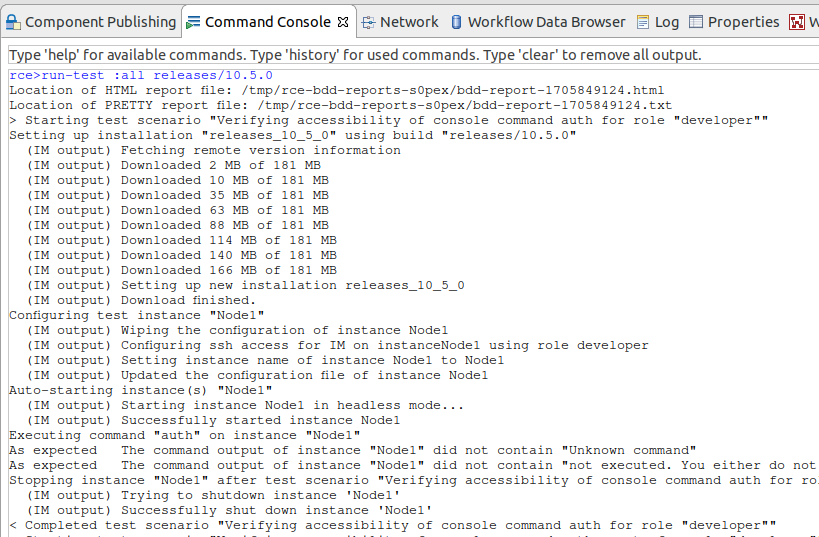
\includegraphics[width=\linewidth]{files/figures/rce-execute-tests.png}
    \caption{Example console output for command: \texttt{run-test :all releases/10.5.0}}
    \label{fig:rce-test-output}
\end{figure}


Although in this step we conducted only a very superficial black-box test through the execution of the tests, we were able to observe two noteworthy aspects. First, the \ac{RCE} tests encompass a diverse range of test cases, covering both functional tests (component, network communication, remote access, etc.) and the \ac{GUI} functionalities. Exclusively in \ac{GUI} tests, \ac{RCE} is launched with an authentic \ac{GUI}, and the functionalities are explicitly emulated through simulated clicks within the \ac{GUI}.
Executing the non-\acs{GUI}-based tests serves as a valuable test case, demonstrating that the typically \acs{GUI} based application can operate successfully without a \acs{GUI}. This testifies that the application can run on a server in a real-world scenario, i.e., without a display server. Additionally, it opens up the possibility of integrating these tests into a CI/CD pipeline, which often lacks the aforementioned display server.

Second, it became apparent that \ac{TSR} relies on \ac{IM} to start multiple \ac{RCE} instances configured as servers or clients. Therefore, we propose that the logic required to simulate a distributed environment is based heavily on the implementation of the \ac{IM} suggesting that it should be further analyzed in a subsequent step.

\subsection{\ac{RCE}'s BDD Testing Setup}
\label{subsec:BuiltinBDDTest}
In this subsection, we illuminate the workings of test execution. Initially, we provide a detailed overview of the setup and execution flow. Following that, we delve into how \ac{RCE} establishes a distributed system comprising multiple \ac{RCE} clients and servers locally. Next, we explain how \ac{RCE} overcomes the challenge of triggering behaviors and obtaining the state to properly evaluate the test cases across multiple clients and servers correctly. Finally, we offer a brief summary and conclusion.

\subsubsection{\ac{RCE}'s Test Setup and Execution Details}
The specifics of the Test Setup are detailed in \ac{RCE}'s Developer Guide~\cite{rceDevGuide10x} and thoroughly discussed in the work by Mischke et al. (2022)~\cite{10.1007/978-3-031-08760-8_44}. In essence, the test setup for \ac{RCE} revolves around the implementation of its test suite through a specialized component, called \acf{TSR}.
Due to its complexity, the whole setup is illustrated in~\Cref{fig:rce-setup}.

\begin{figure}[h]
    \centering
    \includesvg[scale=0.50]{files/figures/RCE-Setup.drawio.svg}
    \caption{Illustration of the interplay between the Test Script Runner (TSR), Instance Management Component (IM), and RCE instances: The TSR functions as a central test runner for the BDD test responsible in executing the test, the IM is used by the TSR and responsible for downloading and managing RCE instances, commands are sent to RCE instances over SSH via the IM.}
    \label{fig:rce-setup}
\end{figure}

The \ac{TSR} component assumes the responsibility of interpreting Gherkin files and executing tests under predefined conditions. To process Gherkin files, \ac{TSR} leverages the Cucumber library~\cite{10.1007/978-3-031-08760-8_44}, facilitating the mapping of free expressions in Gherkin to the corresponding actions executed during tests.

Within Gherkin feature files, the ``GIVEN`` clauses specify, for example, that \ac{TSR} must instantiate multiple client and server instances of \ac{RCE}. This initiation is facilitated by delegating the launch of numerous \ac{RCE} instances via the \acf{IM}~\cite{rceDevGuide10x}. 
The \ac{IM} plays a crucial role in overseeing \ac{RCE} instances used for testing purposes, which includes tasks such as downloading \ac{RCE}, initiating, and terminating instances~\cite{10.1007/978-3-031-08760-8_44,rceDevGuide10x}. Given that the tests can be executed even in a localized environment without a network connection, emphasizing the self-sufficiency of the testing process and providing flexibility in conducting tests in isolated settings without external dependencies, the need for \ac{IM} to instantiate the required instances locally becomes apparent.

This assumption can be easily verified using tools such as Task Manager, Process Hacker, htop, etc. Upon monitoring of the processes running during the tests, it becomes apparent that individual \ac{RCE} instances are instantiated as subprocesses of the primary \ac{RCE} instance. This observation aligns with the test description provided by Mischke et al. (2022)~\cite{10.1007/978-3-031-08760-8_44}. This strategic approach enables \ac{RCE} to emulate a locally distributed system with multiple independent instances, facilitating the testing of the implementation of network communication on the loopback device (i.e.,\texttt{localhost}). Consequently, the necessity of establishing and configuring a distributed system across multiple nodes can be mitigated. However, it is essential to acknowledge that this methodology has inherent limitations, as expounded on~\Cref{sec:results}.

In this context, a question arises regarding the monitoring of autonomous processes by the \ac{TSR} and the subsequent execution of actions on them. Specifically, how does the \ac{TSR} handle the absence of direct access to instances instantiated by itself? This limitation presents a challenge in retrieving the state of these instances for the execution of Gherkin ``THEN`` clauses. Additionally, addressing the need for a mechanism to remotely perform actions on the launched RCE instances becomes imperative for the execution of ``WHEN`` clauses.

\subsubsection{Monitoring and Executing Actions on autonomous RCE instances}
As outlined, individual RCE instances are instantiated as autonomous processes. The encapsulation of these processes, which prohibits direct interaction, necessitates an alternative channel for interaction. Specifically, there must be a mechanism through which the \ac{TSR} can instruct individual instances to establish connections and execute workflows or analogous operations. Furthermore, it is crucial to validate the execution of workflows or the establishment of connections between instances. Given that these processes ideally operate independently within a distributed system, these operations must be performed through network communication.

Examination of the \ac{RCE} Developer and Admin Guide reveals various Command Console commands that offer the required functionality for executing necessary actions and retrieving relevant information~\cite{rceDevGuide10x}. Additionally, instances can be configured for accessibility via \ac{SSH}, enabling the remote execution of commands; without requiring physical access to the machine running RCE~\cite{rceDevGuide10x}. \ac{SSH} operates as a secure, text-based console, allowing encrypted remote communication and device management over unsecured networks~\cite{Schwenk2022}. Hence, executing the aforementioned console commands over \ac{SSH} is crucial, especially when \ac{RCE} functions as a service, running the process in the background (i.e., without \texttt{--console}), thereby avoiding the display of the Command Console. In theory, this \ac{SSH} setup could also be used to address the challenge of accessing the state or executing operations in autonomous \ac{RCE} instances during local tests.

Based on the assumption that the \ac{TSR} utilizes this \ac{SSH} connection for its communication to monitor and control local \ac{RCE} instances, we analyzed the source code and observed that, indeed, \ac{TSR} communicates over \ac{SSH} and extracts all necessary status information from the output of the \ac{SSH} session. In this context, the \ac{TSR} does not create or manage these \ac{SSH} connections itself; instead, this responsibility is delegated to the \ac{IM}. This means that the \ac{TSR} genuinely relies on the \ac{IM} for access and communication with \ac{RCE} instances. Consequently, theoretically transitioning from a local execution approach to a distributed, real-world, cloud-based scenario is straightforward with a simple adjustment of the \ac{IM}.

\subsubsection{Conclusion and Feedback}
In conclusion, RCE features a dedicated component, the \acf{TSR}, which acts as the interface between Gherkin and the execution of tests. It encapsulates all the relevant mappings and business logic required for the execution of tests written in Gherkin. Notably, the logic for initiating and controlling instances is abstracted through the \acf{IM}. \ac{TSR} relies on the \ac{IM} for managing \ac{SSH} connections, delegating responsibility for access and communication with RCE instances. The distribution of the application is facilitated by locally launching multiple RCE instances and controlling them via \ac{SSH}. This approach enables the simulation of a distributed system, providing a more realistic testing environment. It eliminates the need to configure and deploy RCE to an actual distributed system for testing, thus simplifying the local debugging of tests.

A drawback of this setup is that communication over the loopback device rarely exposes network-related error sources. Consequently, testing whether RCE can handle these errors correctly is a challenge. One significant reason for this limitation is that the loopback device provides a virtual network interface exclusively for local communication on the same machine. Therefore, it lacks the complexities and potential issues associated with actual network communication, such as latency, packet loss, and varying network conditions.


Therefore, it would be interesting to explore an alternative approach to simulate network errors, such as inducing latency, packet loss, or network congestion, within the test setup. Examples of such simulations could include introducing artificial delays in communication between \ac{RCE} instances or deliberately dropping packets to assess how \ac{RCE} handles such scenarios. Ideally, executing the tests in a distributed manner, involving individual \ac{RCE} instances in a cluster rather than launching them on a local machine, would provide a more realistic simulation. The abstraction of these tasks by the \ac{IM} makes this theoretically achievable with minimal dependencies due to the abstract implementation of the \ac{IM}. In~\Cref{sec:results}, we present a potential solution to introduce artificial network faults, even within the underlying local setup.

\subsection{Evaluating Fault Tolerance: Provoking Failures in \ac{RCE} Tests}
\label{subsec:fault-tolerance}
This section centers on the evaluation of fault awareness or tolerance within the current suite of \ac{BDD} tests in \ac{RCE}. Our motivation comes from the identification of specific waiting conditions, such as ensuring the successful launch of necessary RCE instances by the \ac{IM}, as mentioned earlier in~\Cref{subsec:PreparingRCETests}. The objective of our examination is to determine the resilience of these waiting conditions, scrutinizing their adaptability to varying system resources, and assessing whether they might contribute to test failures that surpass the predefined wait-for-seconds threshold, because of insufficient resources rather than faulty implementations. An illustrative example of these static waits is presented in~\Cref{lst:staticwait}.

\begin{listing}[!ht]
\caption{Waiting step in Gherkin Scenario}
\label{lst:staticwait}
\inputminted[linenos, xleftmargin=2em]{gherkin}{files/code/staticwait.feature}
\end{listing}

Now, consider the test step in line 4 and it's corresponding implementation, introduced in~\Cref{lst:staticwait_impl}. 

\begin{listing}[!ht]
\caption{Step Definition for waiting step in Gherkin Scenario}
\label{lst:staticwait_impl}
\inputminted[linenos, xleftmargin=2em]{java}{files/code/staticwait_impl.java}
\end{listing}

\begin{listing}[!ht]
\caption{Host System Specs}
\label{lst:host-specs}
\inputminted{text}{files/neofetch-host.txt}
\end{listing}

\begin{listing}[!ht]
\caption{\acl{VM} Guest Specs}
\label{lst:vm-specs}
\inputminted{text}{files/neofetch-test-host.txt}
\end{listing}

In line 7 of the step definition, Java's \texttt{Thread.sleep}\footnote{\seqsplit{https://docs.oracle.com/en/java/javase/11/docs/api/java.base/java/lang/Thread.html}} method is used, that pauses the current thread for at least the specified number of seconds. Using static waits to ensure a desired system state may present challenges, as the predefined time duration might be insufficient and cannot adapt to the available resources in the testing environment. Specifically, the use of static waits can lead to test failures in scenarios where resource availability is limited and required processes cannot be completed within the allocated time. On the other hand, this method may introduce unnecessary delays in test execution when resources are highly efficient and capable of completing tasks more rapidly than expected.

To empirically assess the tolerance of static wait durations under constrained resource conditions, we implemented a controlled experimental setup using a \ac{VM}. The \ac{VM} was hosted on the following bare metal host system, as illustrated in~\Cref{lst:host-specs}. On this system, we set up an Ubuntu 22.04 LTS machine using KVM/QEMU, with the specifications outlined in~\Cref{lst:vm-specs}.

To rule out the presence of faulty tests, we ensured that executing the tests on the system specified in~\Cref{lst:host-specs} led to successful outcomes. In the experimental arrangement in~\Cref{lst:vm-specs}, we intentionally restricted the available resources of the \ac{VM}, notably reducing the RAM to 8 GB and constraining the CPU cores to 2. This was done to emulate an environment characterized by resource insufficiency. By imposing these limitations, our objective was to induce a test failure linked to the static wait issue, utilizing the 5-second threshold depicted in~\Cref{lst:staticwait}. 

While executing all tests on the \ac{VM} system, we observed that despite the short duration of 5 seconds, all ``GIVEN`` clauses were successfully executed. However, a significant number of workflow tests (i.e., \texttt{Workflow05}), failed to complete successfully. Workflow tests denote operations that involve extensive calculations, and the limited number of CPU cores became evident in this context. Upon inspecting the log outputs of the failed tests, we also noted that although the last log output of the test should have been displayed, it was empty. This is likely due to the ongoing computation on the side of the executing \ac{RCE} instance, resulting in a delay in reporting errors or successful messages.

To further investigate the impact of these static waits, we conducted additional tests, including running cpuburn\footnote{https://patrickmn.com/projects/cpuburn/} (similar to Prime95) to simulate increased CPU utilization. Executing a burn test test on our VM, inducing 80\% CPU utilization, resulted in failures in the ``GIVEN`` clauses' waits. It is noteworthy that an 80\% utilization, though seemingly uncommon, could realistically occur in a CI/CD test system with simultaneous execution of multiple tests. Furthermore, the computational performance of these systems may be lower than in our scenario with a single core of the 7940HS, particularly in cloud instances where portions of the cores, i.e. $\frac{1}{8}$, can be allocated to \acp{VM}.

Furthermore, we conducted tests involving manual closure of \ac{RCE} instances instantiated by \ac{IM}. This action aimed to simulate a Java error or crash of \ac{RCE}. Instances terminated in this manner also led to failed tests and were essentially not detected by the \ac{IM}. While this is not inherently problematic, it would be desirable for the \ac{IM} to monitor \ac{RCE} processes through a watchdog and evaluate the shutdown condition accordingly.

\subsection{Code Review of \ac{RCE}'s Testing Setup}
\label{subsec:CodeReview}
To conclude our analysis, we reviewed the source code of both the \ac{TSR} and \ac{IM}. This step was intended to ensure the correctness of the implemented step definitions and their alignment with their intended functionality. It was essential to verify that the step definitions execute the actions as expected and, in the case of ``THEN`` conditions, evaluate them appropriately, avoiding scenarios where, for example, they consistently produce positive evaluations.

During our analysis, we observed that the structure and organization of individual components generally adhere to key code quality principles, such as maintainability, modularity, and reusability. This manifests itself in a clear separation of concerns, as exemplified by the arrangement of the \texttt{\seqsplit{de.rcenvironment.supplemental.testscriptrunner.scripts}} project. Within this project, the feature files describe high-level scenarios, effectively decoupling the overarching behavioral specifications from their underlying implementations, which are stored in the \texttt{\seqsplit{de.rcenvironment.supplemental.testscriptrunner}} project. 

This delineation between the descriptive feature files and the implementation-specific code aligns with best practices in software architecture, promoting clarity and modularity. The adherence to these paradigms is also reflected in the internal structure within each project, ensuring a swift and comprehensible grasp of the project's intricacies. Additionally, it is evident that the business logic is decoupled through interfaces and concrete implementations, allowing the underlying implementations to be dynamically switched if needed. This is particularly positive in the case of \ac{IM}, as described above, which facilitates a relatively straightforward transition from local to remote execution of \ac{RCE} instances. 

One notable observation related to the \ac{IM} was that the \texttt{\seqsplit{InstanceManagementService}} seemed quite tailored to the current structure for local tests, where individual \ac{RCE} instances are downloaded locally by the \ac{IM}. Certain methods, such as \texttt{\seqsplit{getInstallationsRootDir, getVersionOfInstallation}}, and \texttt{getDownloadsCacheDir}, might become obsolete in different configurations. These methods could potentially be implemented without functionality if, for example, the tests are executed on an existing remote cluster, etc. Therefore, this observation is not particularly problematic and serves as a mere observation rather than a significant critique.

However, our analysis identified specific instances that warrant review. Numerous step definitions rely on complex regex patterns, where simpler and more readable Cucumber Expressions could be employed. This is particularly evident in the mapping of test steps within feature files to intricate regular expressions in Cucumber Step Definition annotations (cf. \Cref{fig:cucumber-mapping}). Consequently, this introduces additional cognitive stress for developers, compromising the readability of the code. The resulting complexity poses challenges for immediate comprehensibility, potentially impeding the ease of future modifications and collaborations. Although not pervasive, these readability issues have significance and can potentially impact overall maintainability, especially in scenarios that lack a direct correspondence between the test steps and their definitions.